\documentclass[journal,12pt,twocolumn]{IEEEtran}

\usepackage{enumitem}
\usepackage{amsmath}
\usepackage{amssymb}
\usepackage{gensymb}
\usepackage{graphicx}
\usepackage{txfonts}         
\usepackage{listings}
\usepackage{lstautogobble}
\usepackage{mathtools}
\usepackage{bm}
\usepackage{hyperref}

\newcommand{\solution}{\noindent \textbf{Solution: }}
\providecommand{\pr}[1]{\ensuremath{\Pr\left(#1\right)}}
\providecommand{\brak}[1]{\ensuremath{\left(#1\right)}}
\providecommand{\cbrak}[1]{\ensuremath{\left\{#1\right\}}}
\providecommand{\sbrak}[1]{\ensuremath{\left[#1\right]}}
\providecommand{\mean}[1]{E\left[ #1 \right]}
\providecommand{\var}[1]{\mathrm{Var}\left[ #1 \right]}
\providecommand{\der}[1]{\mathrm{d} #1}
\providecommand{\gauss}[2]{\mathcal{N}\ensuremath{\left(#1,#2\right)}}
\providecommand{\mbf}{\mathbf}
\providecommand{\abs}[1]{\left\vert#1\right\vert}
\providecommand{\norm}[1]{\left\lVert#1\right\rVert}
\providecommand{\z}[1]{{\mathcal{Z}}\{#1\}}
\providecommand{\ztrans}{\overset{\mathcal{Z}}{ \rightleftharpoons}}

\providecommand{\parder}[2]{\frac{\partial}{\partial #2} \brak{#1}}

\let\StandardTheFigure\thefigure
\let\vec\mathbf

\numberwithin{equation}{section}
\renewcommand{\thefigure}{\theenumi}
\renewcommand\thesection{\arabic{section}}

\newcommand{\myvec}[1]{\ensuremath{\begin{pmatrix}#1\end{pmatrix}}}
\newcommand{\mydet}[1]{\ensuremath{\begin{vmatrix}#1\end{vmatrix}}}
\newcommand{\define}{\stackrel{\triangle}{=}}

\DeclareMathOperator*{\argmin}{arg\,min}
\DeclareMathOperator*{\argmax}{arg\,max}

\lstset {
	frame=single, 
	breaklines=true,
	columns=fullflexible,
	autogobble=true
}             
                               
\title{Digital Signal Processing \\ \Large EE3900: Linear Systems and Signal Processing \\ \large Indian Institute of Technology Hyderabad}
\author{Ankit Saha \\ \normalsize AI21BTECH11004 \\ \vspace*{20pt} \normalsize 1 Aug 2022}


\begin{document}

	\maketitle
	
	\section{Software Installation}
	Install the necessary packages by running the following commands
	\begin{lstlisting}
		sudo dnf up
		sudo dnf install libffi-devel libsndfile python3-scipy  python3-numpy python3-matplotlib 
		python -m pip install cffi pysoundfile 
	\end{lstlisting}

	\section{Digital Filter}
	\begin{enumerate}[label=\thesection.\arabic*,ref=\thesection.\theenumi]
	\item \label{prob:input} Download the sound file from  
	\begin{lstlisting}
		wget https://github.com/Ankit-Saha-2003/EE3900/raw/main/Assignment_1/codes/Sound_Noise.wav
	\end{lstlisting}
	
	\item \label{prob:spectrogram} You will find a spectrogram at \href{https://academo.org/demos/spectrum-analyzer}{\url{https://academo.org/demos/spectrum-analyzer}}. Upload the sound file that you downloaded in Problem \ref{prob:input} in the spectrogram  and play.  Observe the spectrogram. What do you find?
	
	\solution There is a lot of background noise and the key strokes are audible. This noise is represented by the large blue and red regions spread from 440 Hz to beyond 18.9 kHz. The key tones are represented by the yellow lines that are present in the lower regions between 440 Hz and 5.1 kHz.
	
	\item \label{prob:output} Write the python code for removal of out of band noise and execute the code. 
	
	\solution Download the python code for the reduction of noise by executing the following command
	\begin{lstlisting}
		wget https://github.com/Ankit-Saha-2003/EE3900/raw/main/Assignment_1/codes/2.3.py
	\end{lstlisting}
	
	Run the code by executing
	\begin{lstlisting}
		python 2.3.py
	\end{lstlisting}
	
	Play the newly created audio file by executing
	\begin{lstlisting}
		aplay Sound_With_Reduced_Noise.wav
	\end{lstlisting}
	
	\item The output of the python script in Problem \ref{prob:output} is the audio file Sound\_With\_Reduced\_Noise.wav. Play the file in the spectrogram in Problem \ref{prob:spectrogram}. What do you observe?
	
	\solution The noise has been reduced considerably and the key strokes are not audible anymore. The blue region is restricted between 440 Hz and 5.1 kHz and there are no signals beyond this range.
	
	
	\end{enumerate}
	
	\section{Difference Equation}
	\begin{enumerate}[label=\thesection.\arabic*,ref=\thesection.\theenumi]
	\item Let
	\begin{equation}
		x(n) = \cbrak{\underset{\uparrow}{1},2,3,4,2,1}
	\end{equation}
	Sketch $x(n)$
	\item Let
	\begin{multline}
		\label{eq:iir_filter}
		y(n) + \frac{1}{2}y(n-1) = x(n) + x(n-2), \\
 		y(n) = 0, n < 0
	\end{multline}
	
	Sketch $y(n)$

	\solution Download the following Python code that plots Fig. \ref{fig-3.2}.
	\begin{lstlisting}
		wget https://github.com/Ankit-Saha-2003/EE3900/raw/main/Assignment_1/codes/3.2.py
	\end{lstlisting}
	
	Run the code by executing
	\begin{lstlisting}
		python 3.2.py
	\end{lstlisting}

	\begin{figure}[!ht]
		\centering
		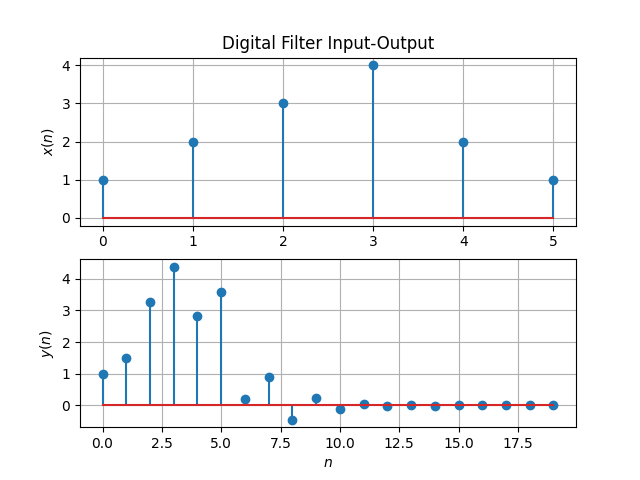
\includegraphics[width=\columnwidth]{./figs/3.2.png}
		\caption{The sketches of $x(n)$ and $y(n)$}
		\label{fig-3.2}	
	\end{figure}
	
	\item Repeat the above exercise using a C code.
	
	\solution Download the following C code that generates the values of $y(n)$
	\begin{lstlisting}
		wget https://github.com/Ankit-Saha-2003/EE3900/raw/main/Assignment_1/codes/3.3.c
	\end{lstlisting}
	
	Compile and run the C program by executing the following
	\begin{lstlisting}
		cc 3.3.c
		./a.out
	\end{lstlisting}
	
	Download the following Python code that plots Fig. \ref{fig-3.3} using the data generated by the above C code
	\begin{lstlisting}
		wget https://github.com/Ankit-Saha-2003/EE3900/raw/main/Assignment_1/codes/3.3.py
	\end{lstlisting}
	
	Run the code by executing
	\begin{lstlisting}
		python 3.3.py
	\end{lstlisting}

	\begin{figure}[!ht]
		\centering
		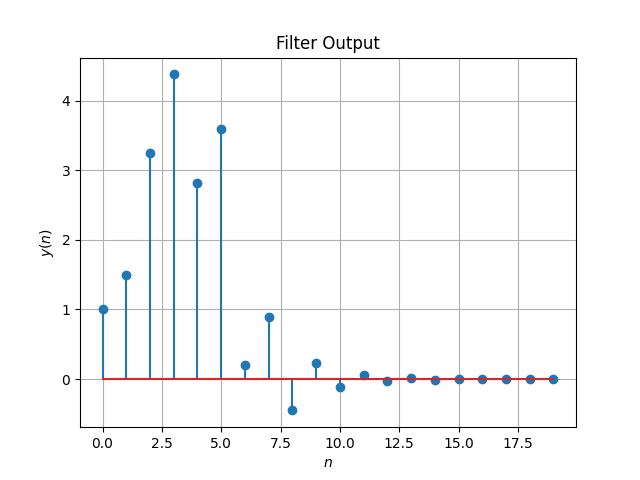
\includegraphics[width=\columnwidth]{./figs/3.3.png}
		\caption{Plot of $y(n)$}
		\label{fig-3.3}	
	\end{figure}
	
	\end{enumerate}
	
	\section{$Z$-transform}
	\begin{enumerate}[label=\thesection.\arabic*]
	\item The $Z$-transform of $x(n)$ is defined as
	\begin{equation}
		\label{eq:z_trans}
		X(z)={\mathcal {Z}}\{x(n)\}=\sum _{n=-\infty }^{\infty }x(n)z^{-n}
	\end{equation}
	Show that
	\begin{equation}
		\label{eq:shift1}
		{\mathcal {Z}}\{x(n-1)\} = z^{-1}X(z)
	\end{equation}
	and find
	\begin{equation}
		{\mathcal {Z}}\{x(n-k)\} 
	\end{equation}
	
	\solution 
	\begin{align}
		{\mathcal {Z}}\{x(n-1)\} &= \sum _{n=-\infty }^{\infty }x(n - 1)z^{-n} 
	\end{align}
	
	Substitute $n - 1 = m$
	\begin{align}
		{\mathcal {Z}}\{x(n-1)\} &=  \sum _{m=-\infty }^{\infty }x(m)z^{-(m+1)} \\
		&= z^{-1} \sum _{m=-\infty }^{\infty }x(m)z^{-m} \\
		&= z^{-1} {\mathcal {Z}}\{x(m)\} \\	
		&= z^{-1} X(z) \\
		{\mathcal {Z}}\{x(n-k)\} &=  \sum _{n=-\infty }^{\infty }x(n - k)z^{-n} \\
		&=  \sum _{m=-\infty }^{\infty }x(m)z^{-(m+k)} \\
		&= z^{-k} \sum _{m=-\infty }^{\infty }x(m)z^{-m} \\
		&= z^{-k} X(z)
	\end{align}	
	
	\item Find
	\begin{equation}
		H(z) = \frac{Y(z)}{X(z)}
	\end{equation}

	from  \eqref{eq:iir_filter} assuming that the $Z$-transform is a linear operation.

	\solution 
	\begin{align}
		y(n) + \frac{1}{2}y(n-1) = x(n) + x(n-2)
	\end{align}
	
	On applying the $Z$-transform on both sides of the equation, we get
	\begin{align}
		{\mathcal {Z}}\cbrak{y(n) + \frac{1}{2}y(n-1)} = {\mathcal {Z}}\{x(n) + x(n-2)\}
	\end{align}
	
	Since we are assuming that the $Z$-transform is a linear operation,
	\begin{align}
		\z{y(n)} + \frac12 \z{y(n-1)} &= \z{x(n)} + \z{x(n-2)} \\
		\implies Y(z) + \frac12 z^{-1} Y(z) &= X(z) + z^{-2} X(z) \\
		\implies Y(z) \brak{1 + \frac12 z^{-1}} &= X(z) (1 + z^{-2}) \\
		\therefore H(z) = \frac{Y(z)}{X(z)} &= \frac{1 + z^{-2}}{1 + \frac12 z^{-1}}
	\end{align}
	
	\item Find the Z transform of 
	\begin{equation}
		\delta(n) =
		\begin{cases}
			1 & n = 0 \\
			0 & \text{otherwise}
		\end{cases}
	\end{equation}
	and show that the $Z$-transform of
	\begin{equation}
	\label{eq:unit_step}
	u(n) =
	\begin{cases}
		1 & n \ge 0 \\
		0 & \text{otherwise}	
	\end{cases}
	\end{equation}
	is
	\begin{equation}
		U(z) = \frac{1}{1-z^{-1}} \quad \abs{z} > 1
	\end{equation}
	
	\solution 
	\begin{align}
		\z{\delta(n)} &= \sum _{n=-\infty }^{\infty }\delta(n)z^{-n} \\
		&= \delta(0) z^{-0} \\
		&= 1 
	\end{align}
	\begin{align}
		\z{u(n)} &= \sum _{n=-\infty }^{\infty } u(n)z^{-n} \\
		&= \sum _{n=0}^{\infty } \brak{z^{-1}}^n 
	\end{align}
	
	This is the sum of an infinite geometric progression with first term $1$ and common ratio $z^{-1}$. The sum converges when
	\begin{equation}
		\abs{z^{-1}} < 1 \iff \abs{z} > 1
	\end{equation}
	
	Therefore,
	\begin{equation}
		U(z) = \z{u(n)} = \frac{1}{1 - z^{-1}} \quad \abs{z} > 1
	\end{equation}

	\item Show that 
	\begin{equation}
		\label{eq:anun}
		a^nu(n) \ztrans \frac{1}{1-az^{-1}} \quad \abs{z} > \abs{a}
	\end{equation}
	
	\solution
	\begin{align}
		\z{a^nu(n)} &= \sum _{n=-\infty }^{\infty } a^nu(n)z^{-n} \\
		&= \sum _{n=0}^{\infty } \brak{az^{-1}}^{n} 
	\end{align}
	
	This is the sum of an infinite geometric progression with first term $1$ and common ratio $az^{-1}$. The sum converges when
	\begin{equation}
		\abs{az^{-1}} < 1 \iff \abs{z} > \abs{a}
	\end{equation}
	
	Therefore,
	\begin{equation}
		\z{a^nu(n)} = \frac{1}{1-az^{-1}} \quad \abs{z} > \abs{a}
	\end{equation}
	
	\item Let
	\begin{equation}
		H\brak{e^{\j \omega}} = H\brak{z = e^{\j \omega}}.
	\end{equation}
	Plot $\abs{H\brak{e^{\j \omega}}}$.  Comment.  $H(e^{\j \omega})$ is known as the {\em Discrete-Time Fourier Transform} (DTFT) of $x(n)$
	
	\solution
	\begin{align}
		H\brak{e^{\j \omega}} &= \frac{1 + e^{-2\j\omega}}{1 + \frac12 e^{-\j\omega}} \\
		\implies \abs{H\brak{e^{\j \omega}}} &= \frac{\abs{1 + \cos2\omega - \j\sin2\omega}}{\abs{1 + \frac12 \cos\omega - \frac12 \sin\omega}} \\
		&= \sqrt{\frac{(1 + \cos2\omega)^2 + (\sin2\omega)^2}{(1 + \frac12 \cos\omega)^2 + (\frac12 \sin\omega)^2}} \\
		&= \sqrt{\frac{2 + 2\cos2\omega}{\frac54 + \cos\omega}} \\
		&= \sqrt{\frac{2(2\cos^2\omega)4}{5 + 4\cos\omega} } \\
		&= \frac{4\abs{\cos\omega}}{\sqrt{5 + 4\cos\omega}}
	\end{align}
	
	Download the following Python code that plots Fig. \ref{fig-4.5}.
	\begin{lstlisting}
		wget https://github.com/Ankit-Saha-2003/EE3900/raw/main/Assignment_1/codes/4.5.py
	\end{lstlisting}
	
	Run the code by executing
	\begin{lstlisting}
		python 4.5.py
	\end{lstlisting}

	\begin{figure}[!ht]
		\centering
		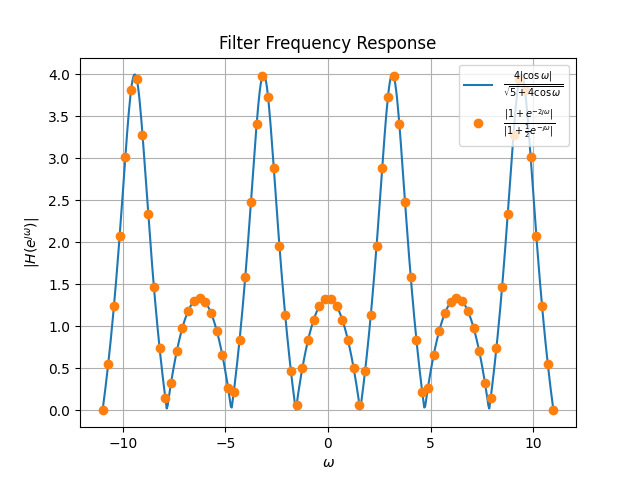
\includegraphics[width=\columnwidth]{./figs/4.5.png}
		\caption{The plot of the magnitude of the discrete-time Fourier transform of $x(n)$}
		\label{fig-4.5}	
	\end{figure}

	From the plot, it is clear that the magnitude of the discrete-time Fourier transform of $x(n)$ is symmetric about $x = 0$ (even function) and is periodic with a period of $2\pi$. 
	
	Also, it attains a maximum value of $4$ at 
	\begin{align}
		x = (2n + 1)\pi, \quad n \in \mathbb{Z}
	\end{align} 
	
	and a minimum of $0$ at 
	\begin{align} 
		x = \brak{2m + 1}\frac{\pi}{2}, \quad m \in \mathbb{Z}\quad 
	\end{align}
	
	\end{enumerate}
	
	\section{Impulse Response}
	\begin{enumerate}[label=\thesection.\arabic*]
	\item \label{prob:impulse_resp}
	Find an expression for $h(n)$ using $H(z)$, given that 
	\begin{equation}
		\label{eq:impulse_resp}
		h(n) \ztrans H(z)
	\end{equation}
	and there is a one to one relationship between $h(n)$ and $H(z)$. $h(n)$ is known as the {\em impulse response} of the system defined by \eqref{eq:iir_filter}
	
	\solution
	\begin{align}
		H(z) &= \frac{1 + z^{-2}}{1 + \frac12 z^{-1}} \\
		&= \frac{1}{1 + \frac12 z^{-1}} + \frac{z^{-2}}{1 + \frac12 z^{-1}}
	\end{align}
	
	From \eqref{eq:anun},
	\begin{align}
		&\frac{1}{1-az^{-1}} \ztrans a^nu(n)  \quad \abs{z} > \abs{a} \\
		\implies &\frac{1}{1 + \frac12 z^{-1}} \ztrans \brak{-\frac12}^n u(n) \quad \abs{z} > \frac12 \\
		\implies &\frac{z^{-2}}{1 + \frac12 z^{-1}} \ztrans \brak{-\frac12}^{n-2} u(n-2) \quad \abs{z} > \frac12
	\end{align}
	
	Since the $Z$-transform is a linear operator, for $\abs{z} > \frac12$
	\begin{align}
		H(z) \ztrans \brak{-\frac12}^n u(n) + \brak{-\frac12}^{n-2} u(n-2)
	\end{align}
	
	Therefore, 
	\begin{align}
		h(n) = \brak{-\frac12}^n u(n) + \brak{-\frac12}^{n-2} u(n-2)
	\end{align}
	
	\item Sketch $h(n)$. Is it bounded? Convergent? 
	
	\solution Download the following Python code that plots Fig. \ref{fig-5.2}.
	\begin{lstlisting}
		wget https://github.com/Ankit-Saha-2003/EE3900/raw/main/Assignment_1/codes/5.2.py
	\end{lstlisting}
	
	Run the code by executing
	\begin{lstlisting}
		python 5.2.py
	\end{lstlisting}

	\begin{figure}[!ht]
		\centering
		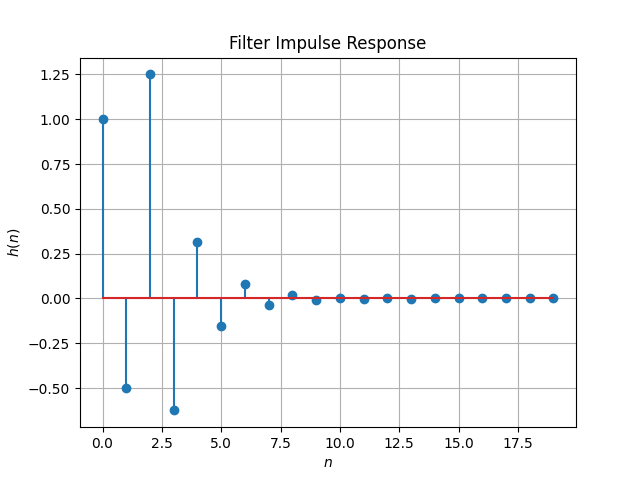
\includegraphics[width=\columnwidth]{./figs/5.2.png}
		\caption{The plot of $h(n)$}
		\label{fig-5.2}	
	\end{figure}
	
	From the plot, it is clear that the sequence is convergent to $0$, which implies that it is bounded as well.
	
	\item The system with $h(n)$ is defined to be stable if
	\begin{equation}
		\sum_{n=-\infty}^{\infty}h(n) < \infty
	\end{equation}
	Is the system defined by \eqref{eq:iir_filter} stable for the impulse response in \eqref{eq:impulse_resp}?	
	
	\solution
	\begin{multline}
		\sum_{n=-\infty}^{\infty}h(n) = \sum_{n=-\infty}^{\infty} \brak{-\frac12}^n u(n) \\
		+ \sum_{n=-\infty}^{\infty} \brak{-\frac12}^{n-2} u(n-2)
	\end{multline}
	\begin{align}
		\sum_{n=-\infty}^{\infty}h(n) = \sum_{n=0}^{\infty}\brak{-\frac12}^n + \sum_{n=2}^{\infty}\brak{-\frac12}^{n-2}
	\end{align}
	
	These are both sums of infinite geometric progressions with first terms $1$ and common ratios $-\frac12$
	\begin{align}
		\sum_{n=-\infty}^{\infty}h(n) &= \frac{1}{1 - \brak{-\frac12}} + \frac{1}{1 - \brak{-\frac12}} \\
		&= \frac{4}{3} < \infty
	\end{align}
	
	Therefore, the system is stable.
	
	\item Compute and sketch $h(n)$ using 
	\begin{equation}
		\label{eq:iir_filter_h}
		h(n) + \frac{1}{2}h(n-1) = \delta(n) + \delta(n-2)
	\end{equation}

	This is the definition of $h(n)$
	
	\solution 
	\begin{equation}
		h(0) = 1
	\end{equation}
	
	Now, for $n = 1$,
	\begin{align}
		h(1) + \frac12 h(0) &= \delta(1) + \delta(-1) = 0 \\
		\implies h(1) &= - \frac{1}{2} h(0) = -\frac{1}{2}
	\end{align}
	
	For $n = 2$,
	\begin{align}
		h(2) + \frac12 h(1) &= \delta(2) + \delta(0) = 1 \\
		\implies h(2) &= 1 - \frac{1}{2} h(1) = \frac{3}{2}
	\end{align}
	
	For $n > 2$, the right hand side of the equation is always zero. Thus,
	\begin{align}
		h(n) &= -\frac{1}{2} h(n-1) \qquad n > 2 \\
		h(3) &= \frac{3}{2} \brak{-\frac12} \\
		h(4) &= \frac{3}{2} \brak{-\frac12}^2 \\
		&~\vdots \\
		h(n) &= \frac{3}{2} \brak{-\frac12}^{n-2}
	\end{align}
	
	Therefore,
	\begin{align}
		h(n) = 
		\begin{cases}
			1 & n = 0 \\
			-\dfrac{1}{2} & n = 1 \\
			\dfrac{3}{2} \brak{-\dfrac12}^{n-2} & n \ge 2
		\end{cases}
	\end{align}
	
	Thus, it is bounded and convergent to $0$
	\begin{equation}
		\lim_{n \to \infty} h(n) = 0
	\end{equation}
	
	Download the following Python code that plots Fig. \ref{fig-5.4}.
	\begin{lstlisting}
		wget https://github.com/Ankit-Saha-2003/EE3900/raw/main/Assignment_1/codes/5.4.py
	\end{lstlisting}
	
	Run the code by executing
	\begin{lstlisting}
		python 5.4.py
	\end{lstlisting}

	\begin{figure}[!ht]
		\centering
		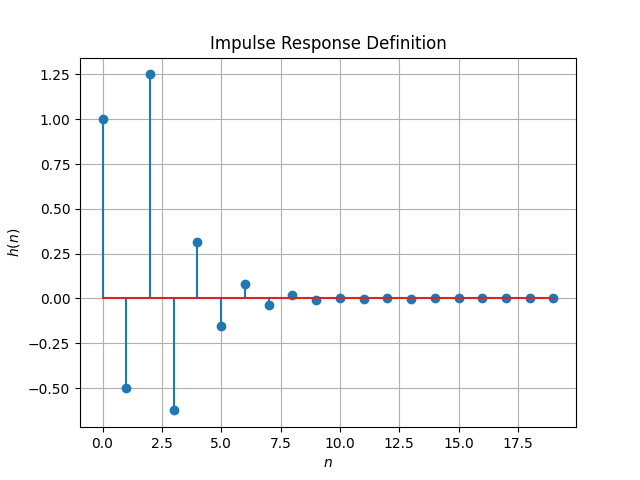
\includegraphics[width=\columnwidth]{./figs/5.4.png}
		\caption{The plot of $h(n)$ from its definition}
		\label{fig-5.4}	
	\end{figure}
	
	\item Compute 
	\begin{equation}
		\label{eq:convolution}
		y(n) = x(n)*h(n) = \sum_{k=-\infty}^{\infty}x(k)h(n-k)
	\end{equation}

	Comment. The operation in \eqref{eq:convolution} is known as {\em convolution}
	
	\solution
	\begin{align}
		x(n)*h(n) &= \sum_{k=-\infty}^{\infty}x(k)h(n-k) \\
		&= \sum_{k=0}^{5}x(k)h(n-k)
	\end{align}
	since $x(k) = 0$ for $k < 0$ and $k > 5$ 
	
	Download the following Python code that plots Fig. \ref{fig-5.5}.
	\begin{lstlisting}
		wget https://github.com/Ankit-Saha-2003/EE3900/raw/main/Assignment_1/codes/5.5.py
	\end{lstlisting}
	
	Run the code by executing
	\begin{lstlisting}
		python 5.5.py
	\end{lstlisting}

	\begin{figure}[!ht]
		\centering
		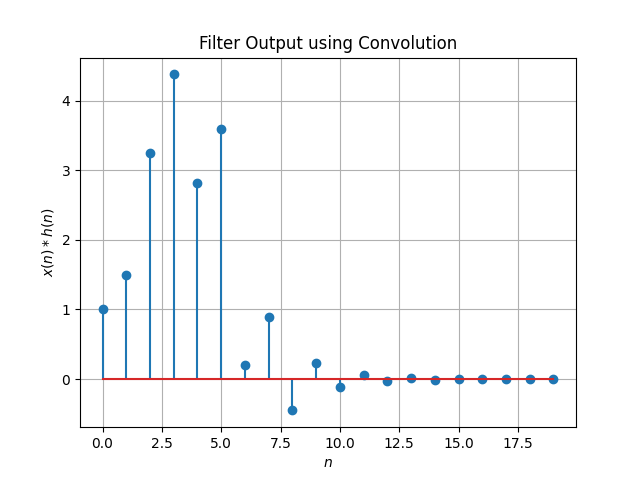
\includegraphics[width=\columnwidth]{./figs/5.5.png}
		\caption{Plot of the convolution of $x(n)$ and $h(n)$}
		\label{fig-5.5}	
	\end{figure}
	
	The plot is exactly the same as that obtained in Fig. \ref{fig-3.2}. Therefore, we can conclude that
	\begin{equation}
		y(n) = x(n)*h(n) 
	\end{equation}
	
	Alternatively, download the following code for computing the convolution by using a Toeplitz matrix
	\begin{lstlisting}
		wget https://github.com/Ankit-Saha-2003/EE3900/raw/main/Assignment_1/codes/5.5-toeplitz.py
	\end{lstlisting}
	
	Run the code by executing
	\begin{lstlisting}
		python 5.5-toeplitz.py
	\end{lstlisting}

	\begin{figure}[!ht]
		\centering
		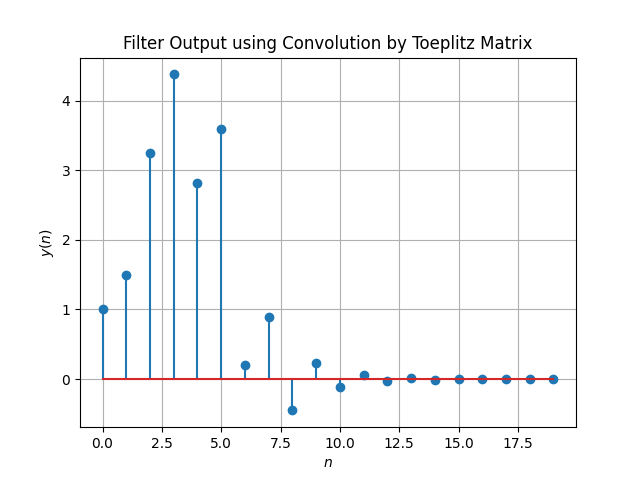
\includegraphics[width=\columnwidth]{./figs/5.5-toeplitz.png}
		\caption{Plot of the convolution of $x(n)$ and $h(n)$}
		\label{fig-5.5-toeplitz}	
	\end{figure}
	
	
	\item Show that
	\begin{equation}
		y(n) =  \sum_{k=-\infty}^{\infty}x(n-k)h(k)
	\end{equation}
	
	\solution We know that
	\begin{equation}
		y(n) = x(n)*h(n) = \sum_{k=-\infty}^{\infty}x(k)h(n-k)
	\end{equation}
	
	Substitute $k = n - i$
	\begin{align}
		 \sum_{k=-\infty}^{\infty}x(k)h(n-k) &=  \sum_{n - i =-\infty}^{\infty}x(n-i)h(n-(n-i)) \\
		 &= \sum_{i = \infty}^{-\infty} x(n - i) h(i) \\
		 &= \sum_{i = -\infty}^{\infty} x(n - i) h(i)
	\end{align}
	since the order of limits does not matter for a summation.
	Thus,
	\begin{align}
		\sum_{k=-\infty}^{\infty}x(k)h(n-k) &= \sum_{k=-\infty}^{\infty}x(n-k)h(k) \\
		\implies x(n) * h(n) &= h(n) * x(n)
	\end{align}
	
	Therefore, convolution is commutative.
	
	\end{enumerate}
	
	\section{DFT and FFT}
	\begin{enumerate}[label=\thesection.\arabic*]
	\item Compute
	\begin{equation}
		X(k) \define \sum _{n=0}^{N-1}x(n) e^{-\j2\pi kn/N} \quad k = 0,1,\dots, N-1
	\end{equation}
	and $H(k)$ using $h(n)$
	
	\solution Download the following Python code that plots Fig. \ref{fig-6.1}.
	\begin{lstlisting}
		wget https://github.com/Ankit-Saha-2003/EE3900/raw/main/Assignment_1/codes/6.1.py
	\end{lstlisting}
	
	Run the code by executing
	\begin{lstlisting}
		python 6.1.py
	\end{lstlisting}

	\begin{figure}[!ht]
		\centering
		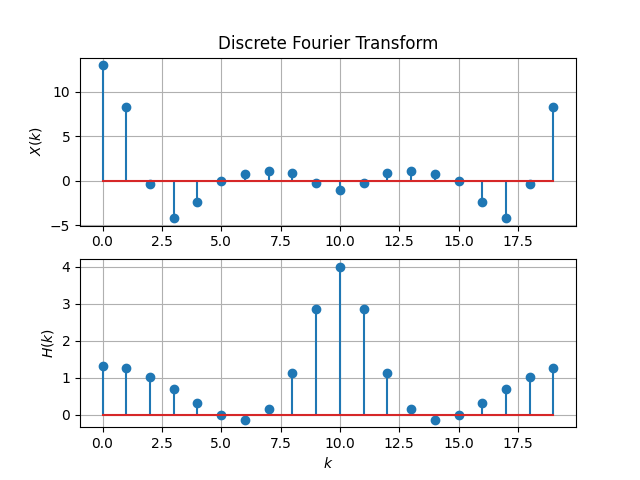
\includegraphics[width=\columnwidth]{./figs/6.1.png}
		\caption{Plots of the real parts of the discrete Fourier transforms of $x(n)$ and $h(n)$}
		\label{fig-6.1}	
	\end{figure}
	
	\item Compute 
	\begin{equation}
		Y(k) = X(k)H(k)
	\end{equation}
	
	\solution Download the following Python code that plots Fig. \ref{fig-6.2}.
	\begin{lstlisting}
		wget https://github.com/Ankit-Saha-2003/EE3900/raw/main/Assignment_1/codes/6.2.py
	\end{lstlisting}
	
	Run the code by executing
	\begin{lstlisting}
		python 6.2.py
	\end{lstlisting}

	\begin{figure}[!ht]
		\centering
		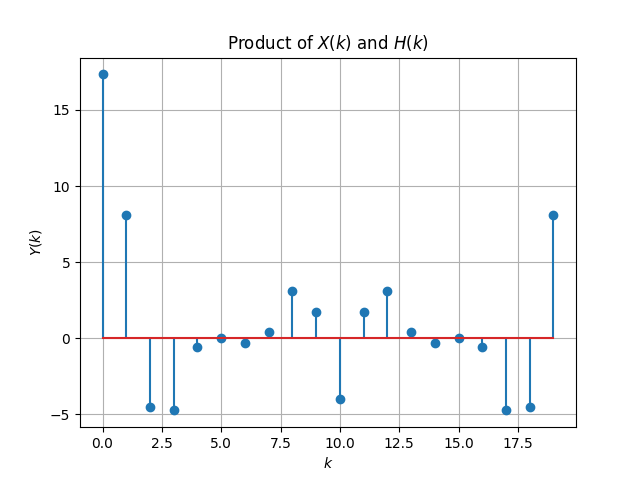
\includegraphics[width=\columnwidth]{./figs/6.2.png}
		\caption{Plot of $Y(k)$}
		\label{fig-6.2}	
	\end{figure}

	\item Compute
	\begin{equation}
 		y\brak{n}={\frac {1}{N}}\sum _{k=0}^{N-1}Y\brak{k}e^{\j 2\pi kn/N} \quad n = 0,1,\dots, N-1
	\end{equation}
	
	\solution Download the following Python code that plots Fig. \ref{fig-6.3}.
	\begin{lstlisting}
		wget https://github.com/Ankit-Saha-2003/EE3900/raw/main/Assignment_1/codes/6.3.py
	\end{lstlisting}
	
	Run the code by executing
	\begin{lstlisting}
		python 6.3.py
	\end{lstlisting}

	\begin{figure}[!ht]
		\centering
		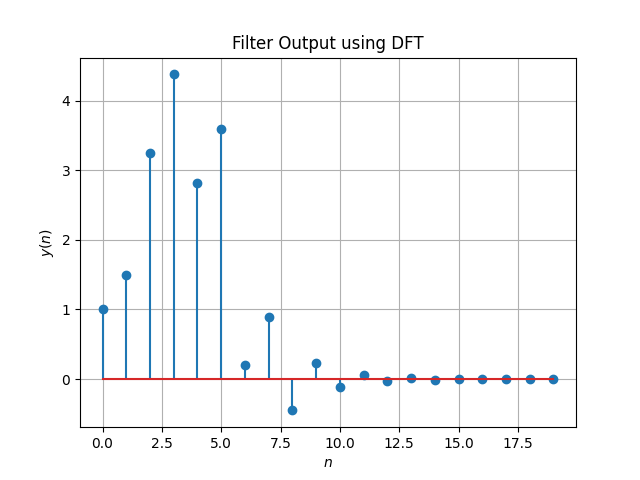
\includegraphics[width=\columnwidth]{./figs/6.3.png}
		\caption{Plot of the inverse discrete Fourier transform of $Y(k)$}
		\label{fig-6.3}	
	\end{figure}
	
	The plot is exactly the same as that obtained in Fig. \ref{fig-3.2}. Therefore, we conclude that 
	\begin{align}
		y(n) &= x(n) * h(n) \\
		\iff Y(k) &= X(k)H(k)
	\end{align}
	
	\item Repeat the previous exercise by computing $X(k), H(k)$ and $y(n)$ through FFT and 
IFFT.
	
	\solution Download the following Python code that plots Fig. \ref{fig-6.4}.
	\begin{lstlisting}
		wget https://github.com/Ankit-Saha-2003/EE3900/raw/main/Assignment_1/codes/6.4.py
	\end{lstlisting}
	
	Run the code by executing
	\begin{lstlisting}
		python 6.4.py
	\end{lstlisting}

	\begin{figure}[!ht]
		\centering
		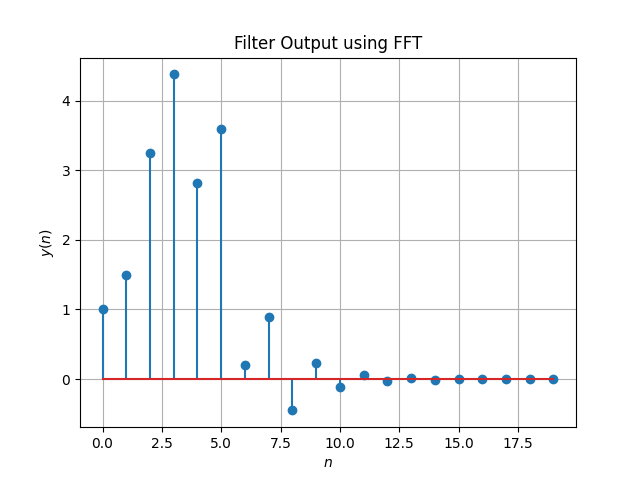
\includegraphics[width=\columnwidth]{./figs/6.4.png}
		\caption{Plot of $y(n)$ by fast Fourier transform}
		\label{fig-6.4}	
	\end{figure}
	
	The plot is exactly the same as that obtained in Fig. \ref{fig-3.2}.
	
	\item Wherever possible, express all the above equations as matrix equations.
	
	\solution
	\begin{align}
		\vec{x} &= \myvec{x_0 & x_1	 & \cdots & x_{N-1}}^\top \\
		\vec{h} &= \myvec{x_0 & x_1	 & \cdots & x_{N-1}}^\top \\
		\vec{y} &= \vec{x} \circledast \vec{h} \\
		\myvec{y_1 \\ y_2 \\ \vdots \\ y_{2N - 1}} &= \myvec{
			h_0 & 0 & 0 & \cdots & 0 \\
			h_1 & h_0 & 0 & \cdots & 0 \\
			h_2 & h_1 & h_0 & \cdots & 0 \\
			\vdots & \vdots & \vdots & \ddots & \vdots \\
			h_{N-1} & h_{N-2} & h_{N-3} & \cdots & h_0 \\
			0 & h_{N-1} & h_{N-2} & \cdots & h_1 \\
			0 & 0 & h_{N-1} & \cdots & h_2 \\
			\vdots & \vdots & \vdots & \ddots & \vdots \\
			0 & 0 & 0 & \cdots & h_{N-1}
		}		
		\myvec{x_1\\x_2\\ \vdots \\x_N}
	\end{align}
	
	The convolution can be written using a Toeplitz matrix. 
	
	Consider the DFT matrix
	\begin{align}
		\vec{W} = \myvec{
			1 & 1 & 1 & 1 & \cdots & 1 \\
			1 & \omega & \omega^2 & \omega^3 & \cdots & \omega^{N-1} \\
			1 & \omega^2 & \omega^4 & \omega^6 & \cdots & \omega^{2(N-1)} \\
			1 & \omega^3 & \omega^6 & \omega^9 & \cdots & \omega^{3(N-1)} \\
			\vdots & \vdots & \vdots & \vdots & \ddots & \vdots \\ 
			1 & \omega^{N-1} & \omega^{2(N-1)} & \omega^{3(N-1)} & \cdots & \omega^{(N-1)(N-1)}
		}
	\end{align}
	
	where $\omega = e^{-\j 2\pi/N}$ is the $N^{\mathrm{th}}$ root of unity
	
	Then the discrete Fourier transforms of $\vec{x}$ and $\vec{h}$ are given by
	\begin{align}
		\vec{X} &= \vec{W} \vec{x} \\
		\vec{H} &= \vec{W} \vec{h}
	\end{align}
	
	$\vec{Y}$ is then given by
	\begin{equation}
		\vec{Y} = \vec{X} \circ \vec{H}
	\end{equation}
	where $\circ$ denotes the Hadamard product (element-wise multiplication)
	
	But $\vec{Y}$ is the discrete Fourier transform of the filter output $\vec{y}$
	\begin{equation}
		\vec{Y} = \vec{W} \vec{y}
	\end{equation}
	
	Thus,
	\begin{align}
		\vec{W} \vec{y} &= \vec{X} \circ \vec{H} \\
		\implies \vec{y} &= \vec{W}^{-1} \brak{\vec{X} \circ \vec{H}} \\
		&= \vec{W}^{-1} \brak{\vec{W} \vec{x} \circ \vec{W} \vec{h}}
	\end{align}
	This is the inverse discrete Fourier transform of $\vec{Y}$

	\end{enumerate}
	
	\section{Exercises}
	Answer the following questions by looking at the python code in Problem \ref{prob:output}
	
	\begin{enumerate}[label=\thesection.\arabic*]
	\item The command
	\begin{lstlisting}
		output_signal = signal.lfilter(b, a, input_signal)
	\end{lstlisting}
	in Problem \ref{prob:output} is executed through the following difference equation
	\begin{equation}
		\label{eq:iir_filter_gen}
 		\sum _{m=0}^{M}a\brak{m}y\brak{n-m}=\sum _{k=0}^{N}b\brak{k}x\brak{n-k}
	\end{equation}
	where the input signal is $x(n)$ and the output signal is $y(n)$ with initial values all 0. Replace \textbf{signal.filtfilt} with your own routine and verify.
	
	\solution 	
	
	\end{enumerate}
\end{document}